\documentclass[12pt,letterpaper]{article}\usepackage[]{graphicx}\usepackage[table]{xcolor}
% maxwidth is the original width if it is less than linewidth
% otherwise use linewidth (to make sure the graphics do not exceed the margin)
\makeatletter
\def\maxwidth{ %
  \ifdim\Gin@nat@width>\linewidth
    \linewidth
  \else
    \Gin@nat@width
  \fi
}
\makeatother

\definecolor{fgcolor}{rgb}{0.345, 0.345, 0.345}
\newcommand{\hlnum}[1]{\textcolor[rgb]{0.686,0.059,0.569}{#1}}%
\newcommand{\hlstr}[1]{\textcolor[rgb]{0.192,0.494,0.8}{#1}}%
\newcommand{\hlcom}[1]{\textcolor[rgb]{0.678,0.584,0.686}{\textit{#1}}}%
\newcommand{\hlopt}[1]{\textcolor[rgb]{0,0,0}{#1}}%
\newcommand{\hlstd}[1]{\textcolor[rgb]{0.345,0.345,0.345}{#1}}%
\newcommand{\hlkwa}[1]{\textcolor[rgb]{0.161,0.373,0.58}{\textbf{#1}}}%
\newcommand{\hlkwb}[1]{\textcolor[rgb]{0.69,0.353,0.396}{#1}}%
\newcommand{\hlkwc}[1]{\textcolor[rgb]{0.333,0.667,0.333}{#1}}%
\newcommand{\hlkwd}[1]{\textcolor[rgb]{0.737,0.353,0.396}{\textbf{#1}}}%
\let\hlipl\hlkwb

\usepackage{framed}
\makeatletter
\newenvironment{kframe}{%
 \def\at@end@of@kframe{}%
 \ifinner\ifhmode%
  \def\at@end@of@kframe{\end{minipage}}%
  \begin{minipage}{\columnwidth}%
 \fi\fi%
 \def\FrameCommand##1{\hskip\@totalleftmargin \hskip-\fboxsep
 \colorbox{shadecolor}{##1}\hskip-\fboxsep
     % There is no \\@totalrightmargin, so:
     \hskip-\linewidth \hskip-\@totalleftmargin \hskip\columnwidth}%
 \MakeFramed {\advance\hsize-\width
   \@totalleftmargin\z@ \linewidth\hsize
   \@setminipage}}%
 {\par\unskip\endMakeFramed%
 \at@end@of@kframe}
\makeatother

\definecolor{shadecolor}{rgb}{.97, .97, .97}
\definecolor{messagecolor}{rgb}{0, 0, 0}
\definecolor{warningcolor}{rgb}{1, 0, 1}
\definecolor{errorcolor}{rgb}{1, 0, 0}
\newenvironment{knitrout}{}{} % an empty environment to be redefined in TeX

\usepackage{alltt}

%%%%% packages
\usepackage{graphicx}
\usepackage{color}
\usepackage[top=1in, bottom=1in, left=1in, right=1in]{geometry}
\usepackage{amsmath,float,hyperref,indentfirst,sectsty,setspace,times}
\hypersetup{colorlinks, allcolors={black}}  % default link color
\hypersetup{pdfpagemode=UseNone} % don't show bookmarks on initial view
\setlength{\rightskip}{0pt plus 1fil} % makes ragged right
\usepackage[authoryear]{natbib}
\bibpunct{(}{)}{;}{a}{}{,}
\usepackage[labelsep=space]{caption}
\usepackage[table]{xcolor}
%%%%%%%%%%%%%%

\allsectionsfont{\normalfont\sffamily\bfseries}
\renewcommand{\figurename}{\textbf{Figure}}
\renewcommand{\thefigure}{\textbf{\arabic{figure}}}
\renewcommand{\tablename}{\textbf{Table}}
\renewcommand{\thetable}{\textbf{\arabic{table}}}



\IfFileExists{upquote.sty}{\usepackage{upquote}}{}
\begin{document}

\setstretch{2.0}

\vspace*{8mm}
\begin{center}

\textbf{\Large A generic hidden Markov model
for multi-parent populations}

\bigskip \bigskip \bigskip \bigskip

{\large Karl W. Broman$^{*,1}$}

\bigskip \bigskip

$^{*}$Department of Biostatistics and Medical Informatics,
University of Wisconsin--Madison, Madison, Wisconsin 53706

\end{center}

%%% Add today's date
\def\todayISO{\leavevmode\hbox{\the\year-\twodigits\month-\twodigits\day}}
\def\twodigits#1{\ifnum#1<10 0\fi\the#1}

\vspace{3in} \hfill {\footnotesize \todayISO}
%%%%%%%%%%%%%%%%%

\clearpage

\noindent \textbf{Running head:} Generic HMM for MPPs


\bigskip \bigskip \bigskip

\noindent \textbf{Key words:} quantitative trait loci, QTL, HMM,
Collaborative Cross, Diversity Outbred mice, heterogeneous stock, MPP,
multiparental populations, Multiparent Advanced Generation Inter-Cross
(MAGIC)



\bigskip \bigskip \bigskip

\noindent \textbf{$^1$Corresponding author:}

\begin{tabular}{lll}
 \\
 \hspace{1cm} & \multicolumn{2}{l}{Karl W Broman} \\
 & \multicolumn{2}{l}{Department of Biostatistics and Medical Informatics} \\
 & \multicolumn{2}{l}{University of Wisconsin--Madison} \\
 & \multicolumn{2}{l}{2126 Genetics-Biotechnology Center} \\
 & \multicolumn{2}{l}{425 Henry Mall} \\
 & \multicolumn{2}{l}{Madison, WI 53706} \\
 \\
 & Phone: & 608--262--4633 \\
 & Email: & \verb|broman@wisc.edu|
\end{tabular}


\clearpage

\section*{Abstract}

A common step in the analysis of multi-parent populations is genotype
reconstruction: identifying the founder origin of haplotypes from
dense marker data. This process often makes use of a probability model
for the pattern of founder alleles along chromosomes, including the
relative frequency of founder alleles and the probability of exchanges
among them, which depend on a model for meiotic recombination and on
the mating design for the population. While the precise experimental
design used to generate the population may be used to derive a precise
characterization of the model for exchanges among founder alleles,
this can be tedious, particularly given the great variety of
experimental designs that have been proposed. We describe an
approximate model that can be applied for a variety of multi-parent
populations. We have implemented the approach in the R/qtl2 software,
and we illustrate its use in applications to publicly-available data
on Diversity Outbred and Collaborative Cross mice.




\clearpage
\section*{Introduction}

Multi-parent populations (MPPs) are valuable resources for the
analysis of complex traits \citep{dekoning2017}, including the mapping
of quantitative trait loci (QTL). A wide variety of MPPs have been
developed, including heterogeneous stock (HS) in mice \citep{mott2000} and
rats \citep{solberg2010}, eight-way recombinant inbred lines (RIL) in mice
\citep{ctc2004} and Drosophila \citep{king2012}, and multi-parent
advanced generation intercross (MAGIC) populations
in a variety of plant species including Arabidopsis \citep{kover2009},
wheat \citep{cavanagh2008}, maize \citep{dellacqua2015}, and rice
\citep{bandillo2013}.

QTL mapping in MPPs can be performed through statistical
tests at individual single nucleotide polymorphisms (SNPs), as used
in genome-wide association studies. However, many investigators
first seek to reconstruct the mosaic of founder haplotypes along the
chromosomes of MPP individuals and use this reconstruction to
test for association between founder alleles and the quantitative
phenotype. This approach was first introduced by \citet{mott2000} for
the analysis of HS mice, implemented in the HAPPY software,
and has been continued in packages such as R/mpMap \citep{huang2011},
DOQTL \citep{gatti2014}, and R/qtl2 \citep{rqtl2}.

The process of genotype reconstruction in an MPP individual is
illustrated in Fig.~\ref{fig1_genome_reconstr}. The genotypes in the
founder strains (Fig.~\ref{fig1_genome_reconstr}\textbf{a}) and the MPP
offspring (Fig.~\ref{fig1_genome_reconstr}\textbf{b}) are used to calculate the
probability of each possible founder genotype at each position along the chromosome
(Fig.~\ref{fig1_genome_reconstr}\textbf{c}). Thresholding of these
probabilities can be used to infer the founder genotypes and the
locations of recombination breakpoints (Fig.~\ref{fig1_genome_reconstr}\textbf{d}).



\begin{figure}
\centering
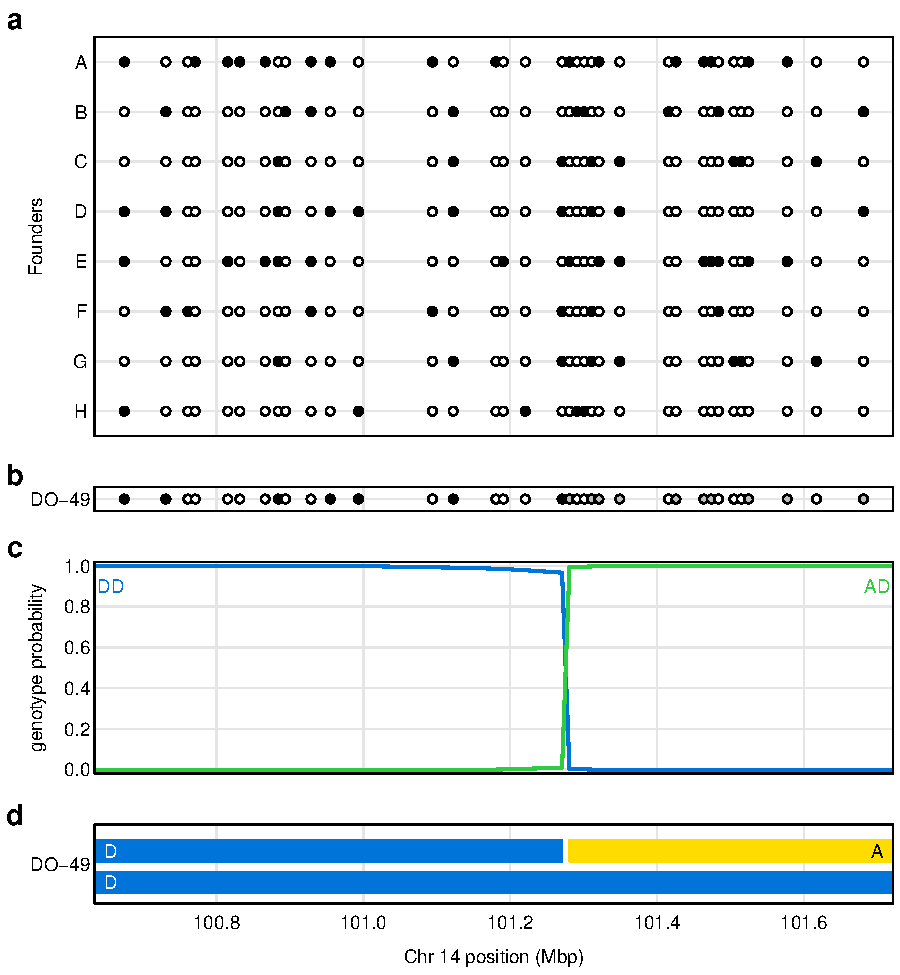
\includegraphics[width=\textwidth]{Figs/fig1_genome_reconstr.pdf}

\caption{Illustration of genotype reconstruction in a 1~Mbp region in
  a single Diversity Outbred (DO) mouse. \textbf{a}.~Genotypes of
  eight founder strains at a set of SNPs, with open and closed circles
  corresponding to being homozygous for the more-frequent and
  less-frequent allele, respectively. \textbf{b}.~Genotype of the DO
  mouse at the SNPs, with gray indicating the mouse is heterozygous.
  \textbf{c}.~Genotype probabilities for the DO mouse along the
  chromosome segment, given the observed data. Genotypes other than
  the two shown have negligible probability across the region.
  \textbf{d}.~Inferred haplotypes in the DO
  mouse.\label{fig1_genome_reconstr}}
\end{figure}





Such genotype reconstructions are valuable not just for QTL analysis
but also for data diagnostics \citep{broman2019}. For example, the
inferred number of recombination breakpoints is a useful diagnostic
for sample quality. Further, the reconstructed genotypes can be used
to derive predicted SNP genotypes; comparing these to the observed SNP
genotypes can help to identify problems in both samples and SNPs.

The probability calculation in Fig.~\ref{fig1_genome_reconstr}\textbf{c}
depends on a model for the process along MPP chromosomes in
Fig.~\ref{fig1_genome_reconstr}\textbf{d}. In the HAPPY software for
HS mice, \citet{mott2000}
used a model of random mating in a large population.
\citet{broman2005} extended the work of \citet{haldane1931}
to derive two-locus genotype probabilities in multi-parent
recombinant inbred lines. This was later developed
for the case of multi-parent advanced intercross populations
\citep{broman2012a,broman2012b}, including Diversity
Outbred (DO) mice \citep{churchill2012}.

Genotype reconstruction for a variety of MPP designs has been
implemented in the R/qtl2 software
\citep[][\url{https://kbroman.org/qtl2}]{rqtl2}. But it can be tedious
analytical work to derive the appropriate transition probabilities
for each new MPP design that is proposed. An alternative is to develop a
more general approach for genotype reconstruction, such as used in the
software RABBIT \citep{zheng2015}. However, this approach has a
variety of parameters that can be difficult to specify.

Here we propose a similarly general method for genotype reconstruction
in MPPs. We imagine that an MPP was derived from a population of
homozygous founder strains at known proportions, $\alpha_i$, followed
by $n$ generations of random mating among a large number of
mating pairs. We can derive the exact transition probabilities for
this situation. The $\alpha_i$ should be simple to specify from the MPP
design, and the effective number of generations of random mating, $n$,
can be determined by computer simulation, to match the expected density of
recombination breakpoints.

Our approach has been implemented in R/qtl2. While we currently focus
on data with SNP genotype calls, such as from microarrays, our model
could potentially be incorporated into methods for genotype imputation
from low-coverage sequencing, such as that of \citet{zheng2018}. We
illustrate our approach through application to publicly-available
datasets on DO \citep{albarghouthi2021} and Collaborative Cross mice
\citep{srivastava2017}.



\clearpage

\section*{Methods}


For genotype reconstruction in a multi-parent population (MPP), we use a
hidden Markov model \citep[HMM; see][]{rabiner1989}. Our basic approach
is as described in \citet[App. D]{rqtlbook} for a biparental
cross; the extension to an MPP is straightforward and described below.

Consider an MPP derived from $k$ inbred lines. We focus on a single
individual, and on a single chromosome with $M$ marker positions
(including pseudomarkers: positions between markers at which we have
no data but would like to infer the underlying genotype). Let $G_m$ be
the underlying genotype at position $m$.
In a homozygous population, such as RIL, the $G_m$ take one of $k$
possible values, the $k$ homozygous genotypes.
In a heterozygous population, such as advanced intercross lines (AIL),
the $G_m$ take one of $\binom{k}{2} + k$ possible values, the
$\binom{k}{2}$ heterozygotes and $k$ homozygotes.
Let $O_m$ be the observed SNP genotype at position $m$
(possibly missing). We assume that the $G_m$ form a Markov chain (that
$G_1, \dots, G_{m-1}$ are conditionally independent of $G_{m+1}, \dots,
G_M$, given $G_m$), and that $O_m$ is conditionally independent of
everything else, given $G_m$. The forward-backward algorithm
\citep[see][]{rabiner1989} takes advantage of
the conditional independence structure of the HMM to calculate
$\Pr(G_m | \boldsymbol{O})$.

The key parameters in the model are the \emph{initial\/}
probabilities, $\pi_g = \Pr(G_1 = g)$, the \emph{transition\/}
probabilities, $t_m(g, g') = \Pr(G_{m+1} = g' \ | \ G_m = g)$, and the
\emph{emission\/} probabilities, $e_m(g) = \Pr(O_m | G_m = g)$. A
particular advantage of the HMM for genotype reconstruction is the
easy incorporation of a model for genotyping errors
\citep{lincoln1992}, which is done through the emission probabilities,
which condition on the founder SNP genotypes but allow some fixed
probability $\epsilon$ that the observed SNP genotype in the MPP
individual is in error and incompatible with the underlying genotype
$G_m$ and the SNP genotypes in the founder lines.

The initial and transition probabilities govern the underlying Markov
chain, including the relative frequency of founder alleles and the
frequency of recombination breakpoints along MPP chromosomes. In
principle, these probabilities may be derived on the basis of the
crossing design for the MPP. In practice, the
transition probabilities can be tedious to derive, and exact
calculations may provide no real advantage for genotype
reconstruction.

Here, we derive the transition probabilities for a generic MPP design,
which may then be applied generally. We consider a founder population
with $k$ inbred lines in proportions $\alpha_i$, and imagine
subsequent generations are produced by random mating with a very large
set of mating pairs.

Consider a pair of loci separated by a recombination fraction of $r$
(assumed the same in both sexes) and let $p_{ij}^{(n)}$ be the
probability of that a random haplotype at generation $n$
has alleles $i$ and $j$.
At $n=0$, we have just the founding inbred lines, and so
$p_{ij}^{(0)} = \alpha_i$ if $i=j$ and $=0$ if $i
\ne j$.

The probabilities from one generation to the next are related by a
simple recursion, as in \citet{broman2012b}. Consider a random haplotype
at generation $n$. It was either a random haplotype from generation
$n-1$ transmitted intact without recombination, or it is a recombinant
haplotype bringing together two random alleles. Thus

\begin{equation}
p_{ij}^{(n)} = (1-r)p_{ij}^{(n-1)} + r \alpha_i \alpha_j
\end{equation}

Using the same techniques described in \citet{broman2012b}, we find
the solutions:

\begin{equation}
  p_{ij}^{(n)} =
\left\{ \begin{array}{ll}
\alpha_i^2 + (1-r)^n \alpha_i (1-\alpha_i) & \quad \text{if } i = j \\
\alpha_i \alpha_j [1 - (1-r)^n]            & \quad \text{if } i \ne j
\end{array}
\right.
\label{eqn:p_ij}
\end{equation}

The transition probabilities along a haplotype are derived by dividing
the above by the marginal probability, $\alpha_i$. Thus if $G_1$ and
$G_2$ are the genotypes at the two loci, we have the following
transition probabilities.

\begin{eqnarray}
\Pr(G_2=j \ | \ G_1=i) =
\left\{ \begin{array}{ll}
\alpha_i + (1-r)^n (1 - \alpha_i) & \quad \text{if } i = j \\
\alpha_j [1 - (1-r)^n]            & \quad \text{if } i \ne j
\end{array}
\right.
\end{eqnarray}

For a heterozygous population (such as heterogeneous stock or
Diversity Outbred mice), an individual will have two random such
haplotypes. For homozygous population (such as MAGIC), we treat them like
doubled haploids, by taking a single random chromosome and doubling
it.

For the X chromosome, we use the same equations but replace $n$ with
$(2/3)n$, since recombination occurs only in females, so in 2/3 of the
X chromosomes. This provides a remarkably tight approximation.

You can potentially use the expected number of crossovers to calibrate
the number generations of random mating, or the map expansion, which
is the relative increase in the number of crossovers. Let $R(r)$ be
the chance that a random haplotype has an exchange of alleles across
an interval with recombination fraction $r$, so $R(r) = 1 - \sum_i
p_{ii}^{(n)}$. The map expansion is $dR/dr$ evaluated at $r=0$
\citep[see][]{teuscher2007}. Using equation~(\ref{eqn:p_ij}) above, we
then get that the map expansion in this population is $n (1 -
\sum\alpha_i^2)$. In the special case that $\alpha_i \equiv 1/k$ for
all $i$, this reduces to $n (k-1)/k$.

The map expansion at generation $s$ in DO mice on an autosome is
$(7/8)(s-1) + M_1$ where $M_1$ is the weighted average of map
expansion in the pre-CC founders \citep{broman2012b}, or about $(7s +
37)/8$. Equating this with $(7/8)n$, we can thus take $n \approx s +
5$ when using this model to approximate the DO. For the Collaborative
Cross, \citet{broman2005} showed that R = 7r/(1+6r), and so the map
expansion is 7. Thus we can take $n=8$ as the effective number of
generations of random mating.


\clearpage
\section*{Applications}

We illustrate our approach with application to datasets on Diversity
Outbred mice \citep{albarghouthi2021} and Collaborative Cross (CC) mice
\citep{srivastava2017}. In both cases, the approach provided results
that were generally equivalent to those from the more exact model, though with
important differences in the results for the X chromosome in the
CC application.

\subsection*{Diversity Outbred mice}



The Diversity Outbred mouse data of \citet{albarghouthi2021} concerns
a set of 619 mice from DO generations
23--33,
in 11 batches by generation
and including 304 females and
315 males. The mice were genotyped on
the GigaMUGA array \citep{morgan2016} and the cleaned data consist of
genotypes at 109,427 markers. A wide variety
of phenotypes are available; we focus on the 20
contributing to the results in Table~1 of \citet{albarghouthi2021}.

We performed genotype reconstruction using the transition matrices
derived specifically for DO mice \citep{broman2019} as well as by the
approximate model proposed above. For the DO mice at generation $n$,
we used the transition probabilities for general 8-way advanced
intercross lines (AIL) at $n+5$.

Following \citet{albarghouthi2021},
we assumed a 0.2\% genotyping error rate and used the Carter-Falconer
map function \citep{carter1951}. Calculations were performed in R
\citep{rcore} with R/qtl2 \citep{rqtl2}, on an 8-core Linux laptop with
64 GB RAM. The calculations with the DO-specific model took
approximately 35 min, while those with the general AIL model took
27 min, an almost 25\% reduction in computation time.

The transition probabilities used by the two models are only subtly
different and become less different in later generations. The
probability of an exchange across an interval on a random DO
chromosome, as a function of the recombination fraction for the
interval and the number of generations, is shown in
Fig.~\ref{fig2_do_trmatrix}.

\begin{figure}
\centering
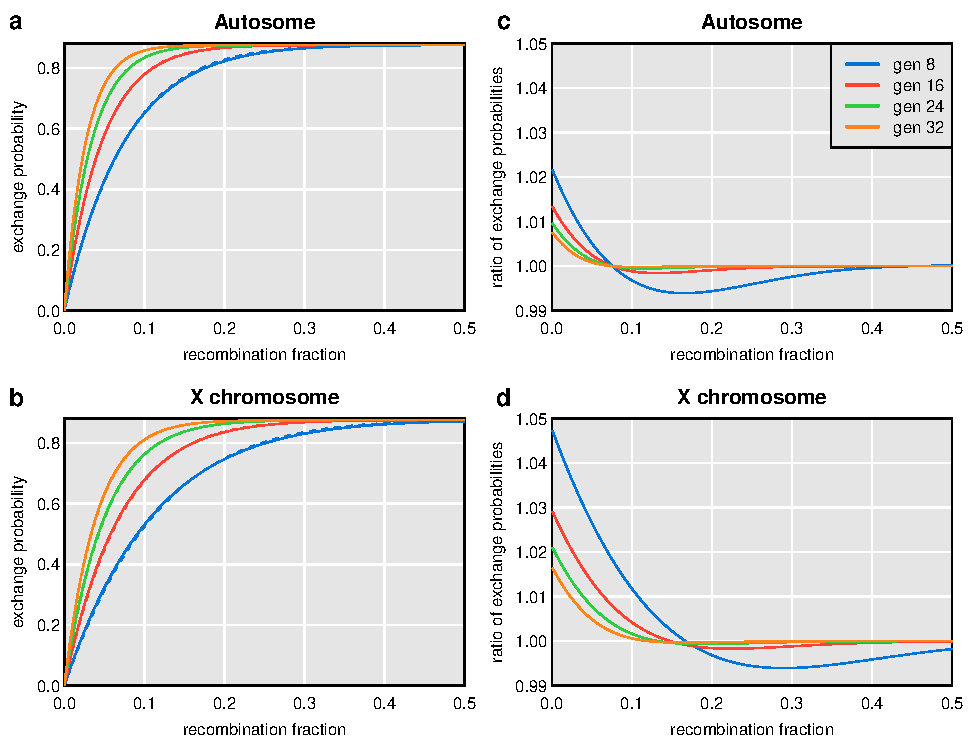
\includegraphics[width=\textwidth]{Figs/fig2_do_trmatrix.pdf}

\caption{Differences in transition probabilities for Diversity
  Outbred mice from more-exact calculations and the proposed
  approximations. Probability of an exchange of alleles
  across an interval as a function of generation with the more-exact
  calculations (solid lines) and the proposed approximation (dashed
  lines) for
  autosomes (\textbf{a}) and the X chromosome (\textbf{b}).
  Ratio of the probabilities (more-exact versus approximation) for
  autosomes (\textbf{c}) and the X chromosome (\textbf{d}).
  \label{fig2_do_trmatrix}}
\end{figure}




QTL analysis proceeded by the method described in \citet{gatti2014}
and also used by \citet{albarghouthi2021}. Namely, we fit a linear
mixed model assuming an additive model for the founder haplotypes,
with a residual polygenic effect to account for relationships among
individuals with kinship matrices calculated using the
``leave-one-chromosome-out'' (LOCO) method \citep[see][]{yang2014},
and with a set of fixed-effect covariates defined in
\citet{albarghouthi2021}.

The genotype probabilities were almost indistinguishable. The maximum
difference was 0.011 on the
X chromosome followed by a difference of
0.007 on chromosome
8.
For that reason, the QTL mapping results were
hardly different. Across all 20 traits considered,
the maximum difference in LOD scores in the two sets of results was
0.02.

The LOD curves by the two methods for tissue mineral density (TMD) and
the differences between them are shown in Fig.~\ref{fig3_do_qtl}. The
QTL on chromosomes 1 and 10 have LOD scores of
23.9
and 14.6,
respectively, but the maximum difference in LOD, genome-wide, between the two
methods is just 0.014.


\begin{figure}
\centering
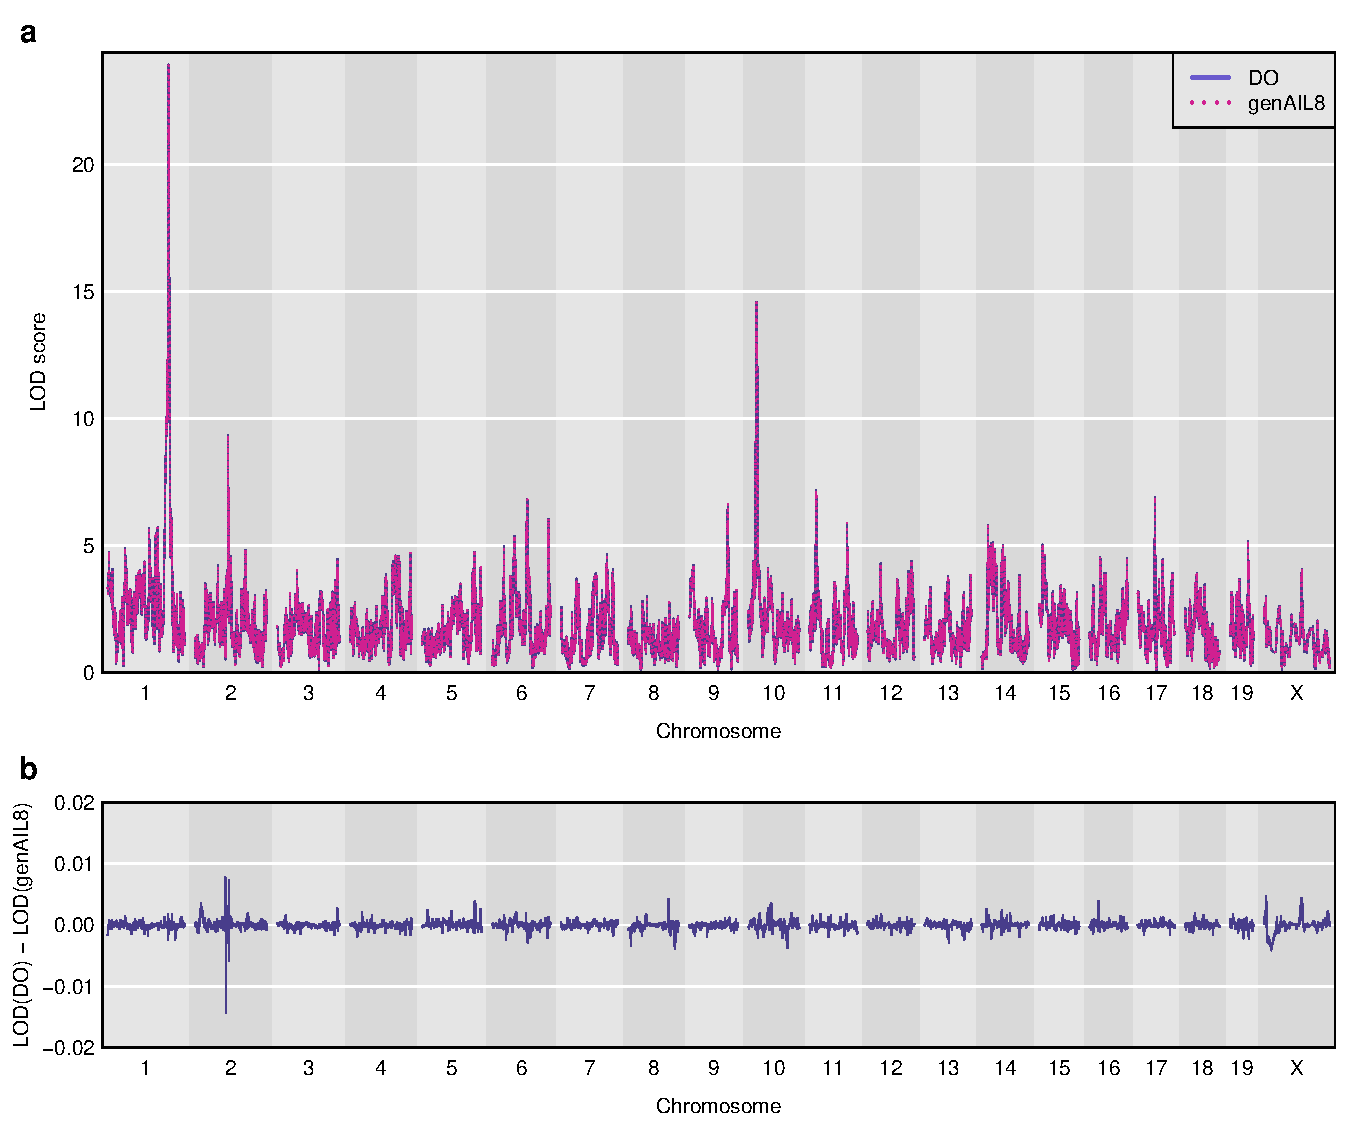
\includegraphics[width=\textwidth]{Figs/fig3_do_qtl.pdf}

\caption{Genome scan for tissue mineral density (TMD) for the DO mouse data
  from \citet{albarghouthi2021}. \textbf{a}. LOD curves across the
  genome using the genotype probabilities from the DO-specific model
  (solid blue curves) and the proposed general model (dotted pink
  curves). \textbf{b}. Differences between the two sets of LOD curves.
  \label{fig3_do_qtl}}
\end{figure}





\subsection*{Collaborative Cross mice}



As a second application of our approach, we consider the data for a
set of 69 Collaborative Cross (CC) lines \citep{srivastava2017}. These are
eight-way recombinant inbred lines (RIL) derived from the same eight
founders as the DO mice, as the DO was formed from 144
partially-inbred lines from the process of developing the CC
\citep{svenson2012}.

Each CC line was formed from a separate ``funnel,'' bringing the
eight founder genomes together as rapidly as possible, for example
[(A$\times$B)$\times$(C$\times$D)]$\times$[(E$\times$F)$\times$(G$\times$H)],
where the female parent is listed first in each cross. Inbreeding was
accomplished by repeated mating between siblings.

The recombination probabilities for the autosomes in the CC do not
depend on the order of the founders in the funnel for a line
\citep{broman2005}. This is in contrast with the case of 8-way RIL by
selfing \citep[see][Table 2]{broman2005}. For the X chromosome,
however, the cross order is important, as only 5 of the 8 founders can
contribute. For example, in a line derived from the cross
[(A$\times$B)$\times$(C$\times$D)]$\times$[(E$\times$F)$\times$(G$\times$H)],
the single-locus genotype probabilities on the X chromosome are 1/6
each for alleles A, B, E, and F, and 1/3 for allele C, while alleles
D, G, and H will be absent. And note that the mitochondrial DNA will
come from founder A, while the Y chromosome will be from founder H.



The cross funnel information was missing for 14
of the 69 CC lines. While the sources of the
mitochondria and Y chromosome were provided for all lines, there were
several inconsistencies in these data: line CC013/GeniUnc has the
same founder listed as the source for its mitochondria and Y
chromosome, and for three lines
(CC031/GeniUnc, CC037/TauUnc, and CC056/GeniUnc) the founder on the Y chromosome is also
seen contributing to the X chromosome.
We used the genotype probabilities reported in
\citet{srivastava2017} to construct compatible cross funnels,
with small modifications to handle the inconsistent information.

We performed genotype reconstruction using the transition matrices
derived specifically for CC mice \citep{broman2005} as well as by the
approximate model proposed above, using $n=8$ generations of random
mating, chosen to match the expected frequency of recombination breakpoints.

The resulting probabilities were nearly identical on all autosomes in
all CC lines. The maximum difference in probabilities on the autosomes
was just 0.0006.

There were some important differences on the X chromosome, however.
There were no cases with high probability pointing to different
founder alleles by the two models, but there were several cases where
two or more founders cannot be distinguished, but some would be
excluded by the assumed cross design.



For example, in Figure~\ref{fig4_cc_xchr}, we show the genotype
probabilities along the X chromosome for strain CC038/GeniUnc, as calculated with
the more-exact model (Figure~\ref{fig4_cc_xchr}\textbf{a}) and with the approximate
model (Figure~\ref{fig4_cc_xchr}\textbf{b}). We also include the results for
the case that the more-exact model but when an incorrect cross design was used
(Figure~\ref{fig4_cc_xchr}\textbf{c}). Note the segment near 135 Mbp, which is
inferred to be from founder NOD with the more-exact model but is equally likely B6
or NOD with the approximate model; the B6 and NOD founder strains are
identical in the region, but the assumed cross design for the
CC038/GeniUnc strain excluded B6. For the results using the incorrect
cross design (which excluded not just B6 but also 129 and NOD), the
results across the entire chromosome become a chopped-up mess,
with an apparent 39 recombination breakpoints, versus
5 when the correct cross information is used.

\begin{figure}
\centering
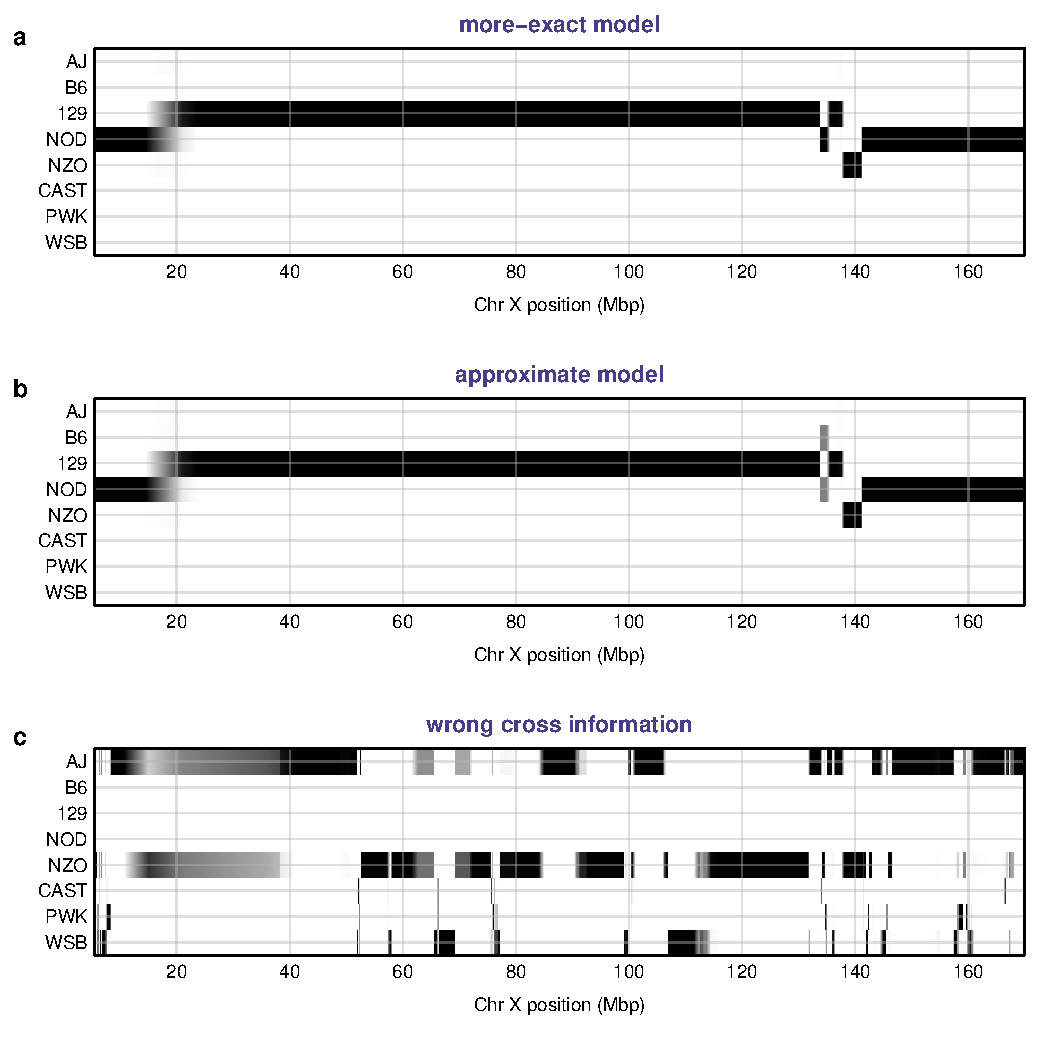
\includegraphics[width=\textwidth]{Figs/fig4_cc_xchr.pdf}

\caption{Genotype probabilities along the X chromosome for Collaborative
  Cross strain CC038/GeniUnc. \textbf{a}. Results using
  the more-exact model that excludes founders
  B6, CAST, and WSB.
  \textbf{b}. Results using the proposed approximate model.
  \textbf{c}. Results using the more-exact model but with the wrong
  cross information, excluding founders
  B6, 129, and NOD.
  \label{fig4_cc_xchr}}
\end{figure}

Overall, there were seven strains
where the maximum difference in the probabilities from the more-exact
model and the proposed approximate model were in the range
0.25 -- 0.50,
and another eight strains with maximum
difference in the range 0.10 -- 0.25. All of the differences concern
cases where multiple founders are identical for a region and either some would
be excluded by the cross design, or where the difference in prior
frequencies affects the results. For example, in the cross
[(A$\times$B)$\times$(C$\times$D)]$\times$[(E$\times$F)$\times$(G$\times$H)],
the frequency of the C allele on the X chromosome is twice that of A,
B, E, and F.










\clearpage
\section*{Discussion}


We have proposed an approximate model for use with genotype
reconstruction in multi-parent populations (MPPs). We derived the
two-point probabilities on autosomes in the case of random mating in
large, discrete generations, derived from a founder population of a
set of inbred lines in known proportions. We use the same frequencies
for the X chromosome, but with 2/3 the number of generations. The
approach is shown to give equivalent results for the mouse DO and CC
populations, though with important differences for the X chromosome in
CC lines, where some founder alleles can be excluded based on the
cross design. The more-exact model for the X chromosome in the CC
excludes three of the eight founders based on the cross design. This
is particularly useful in cases that multiple founders are identical
by descent across a region. However, the approximate model is not
affected by errors in the specified cross design (see Figure~4).

The value of this generic model points towards the general usefulness
of the original software for multi-parent populations, HAPPY
\citep{mott2000}, developed for the analysis of mouse heterogeneous
stock. The results may depend on marker density and informativeness,
but with a dense set of informative markers, a generic approach can
provide good-quality genome reconstructions.

The hidden Markov model itself is an approximation. Meiosis generally
exhibits positive crossover interference, but the Markov property is
closer to being correct in multi-parent populations with multiple
generations of mating, because nearby recombination events come from
independent generations. This was apparent in the
3-point probabilities derived by \citet{haldane1931} for two-way RIL
and was further explored in \citet{broman2005} for multi-way RIL.

The proposed method has been implemented in the R/qtl2 software
\citep{rqtl2}. It requires specification of the founder proportions
and one other parameter (the number of generations of random mating)
which governs the frequency of recombination breakpoints. The founder
proportions should be straightforward from the cross design; the
effective number of generations of random mating may require some
calibration, such as through computer simulation to match the expected
frequency of recombination breakpoints.



\clearpage
\subsection*{Data and software availability}

The R/qtl2 software is available at the Comprehensive R Archive
Network (CRAN), \url{https://cran.r-project.org/package=qtl2}, as well
as GitHub, \url{https://github.com/rqtl/qtl2}. Further documentation
is available at the R/qtl2 website, \url{https://kbroman.org/qtl2}.

The Diversity Outbred mouse data from \citet{albarghouthi2021} is
available at Zenodo, \url{https://doi.org/10.5281/zenodo.4265417}.
Also see their companion repository of analysis scripts at GitHub,
\url{https://github.com/basel-maher/DO_project},
and archived at Zenodo, \url{https://doi.org/10.5281/zenodo.4718146}.

The Collaborative Cross mouse data from \citet{srivastava2017} is
available at Zenodo, \url{https://doi.org/10.5281/zenodo.377036}.
Reorganized files in R/qtl2 format are at
\url{https://github.com/rqtl/qtl2data/tree/main/CC}.

Our detailed analysis code is available at GitHub,
\url{https://github.com/kbroman/Paper_GenericHMM},
and archived at Zenodo, \url{https://doi.org/10.5281/zenodo.5718739}.


\section*{Acknowledgments}

Two anonymous reviewers provided valuable comments for improvement of
the manuscript.



\section*{Funding}

This work was supported in part by
National Institutes of Health grant R01GM070683.



\section*{Conflicts of interest}

The author declares that there is no conflict of interest.




\clearpage
\bibliographystyle{genetics}
\renewcommand*{\refname}{\normalfont\sffamily\bfseries Literature Cited}
\bibliography{gen_hmm}




\end{document}
